\subsection{Non-reflecting boundary conditions}
Finally, we are going to apply non reflecting conditions at the boundaries. As explained in Leveque chapter 7, we extrapolate the variables at the ghost cells by saying :
\begin{align*}
h_0 &= h_1\\
h_N &= h_{N+1}\\
v_0 &= v_1 \implies hv_0 = hv_1\\
v_N &= v_{N+1} \implies hv_N = hv_{N+1}
\end{align*}

Intuitively, the flow is going to "go out" of the domain with such boundary conditions.

The code is available at the end of the report. The structure does not change much, the only difference is the computations of the values of the ghost cells.

Figure \ref{noRe} shows the results when applying the extrapolation for the ghost cells. We can see that at first nothing changes from the original problem. This is coherent since we only changed the boundary conditions . But the waves go out of the domain when reaching the boundaries. This is exactly what we wanted ! There is no reflection noticeable. To investigate a bit more, we can compute the integral of the height on the domain. At $t=2.1$, this value is 10 with accuracy up to floating point errors so we can be sure that there is no reflection at all.

\begin{figure}
\begin{center}
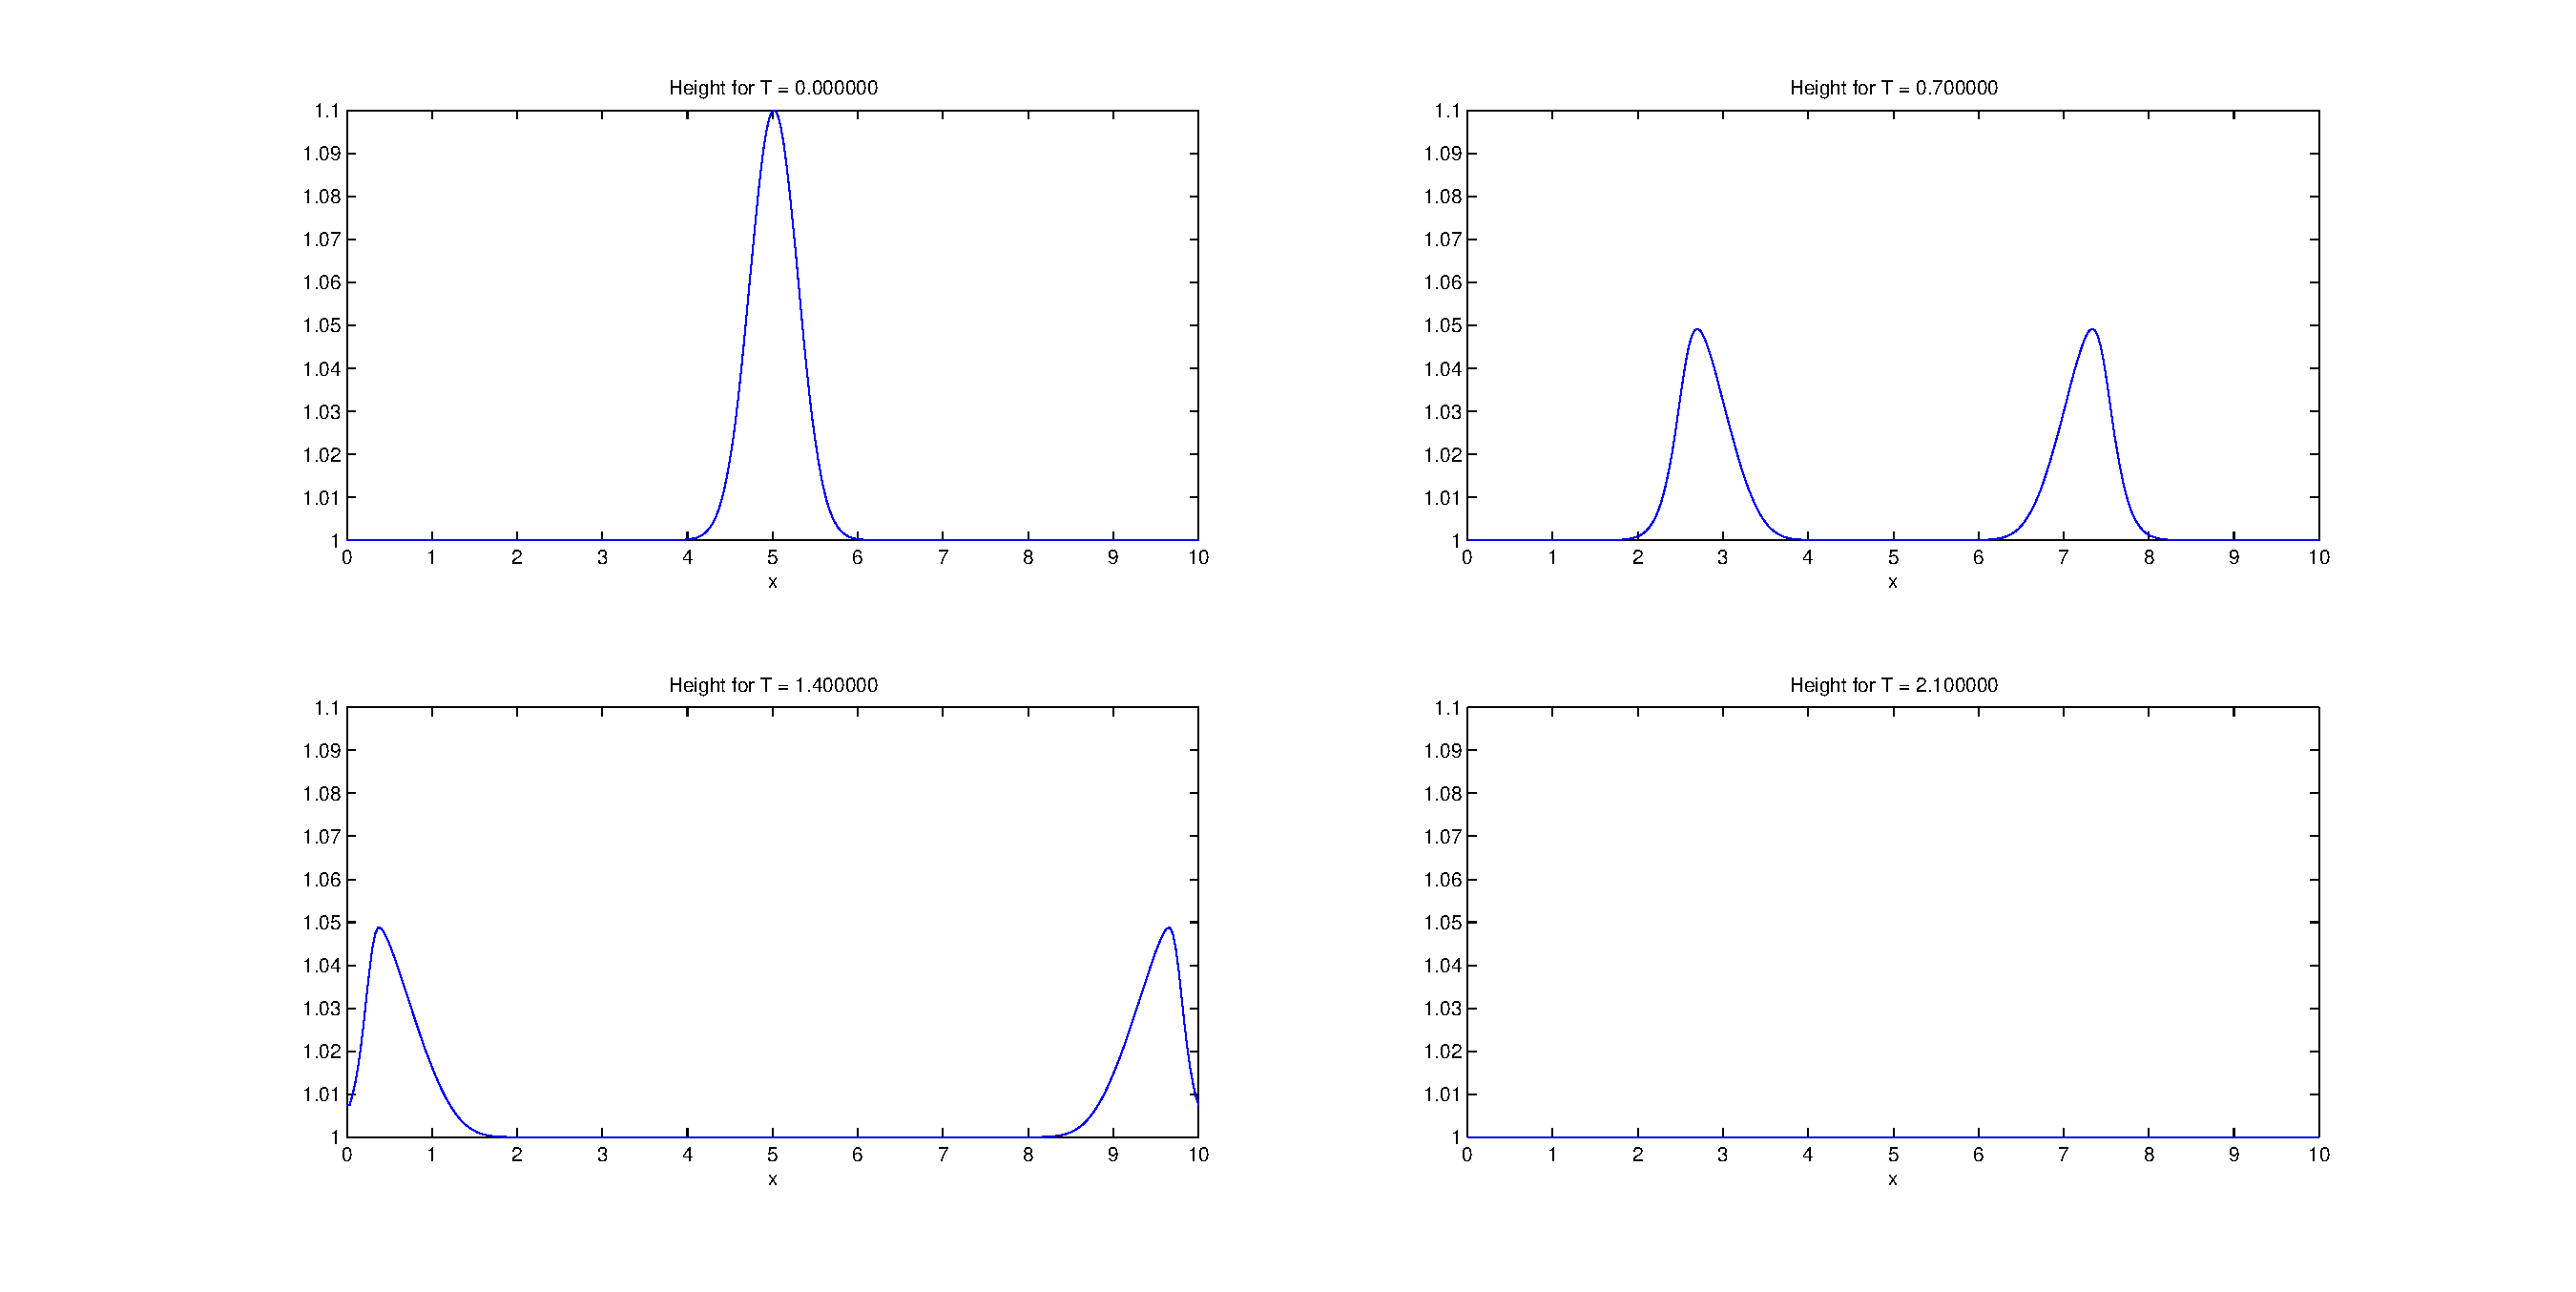
\includegraphics[scale=0.4]{noRe.eps}
\caption{Results with non reflective boundary conditions}
\label{noRe}
\end{center}
\end{figure} 